\documentclass[a4j,titlepage]{jarticle}
\usepackage[dvipdfmx]{graphicx}
\usepackage{ascmac}
\usepackage{url}


\title{呑兵衛土佐巡\\
外部設計書\\
第2版}
\author{株式会社Spirytus}
\date{\today}

\begin{document}
\maketitle
\tableofcontents

\clearpage

\section{機能概要}
\subsection{お酒検索機能}
お酒検索機能では、上記の検索項目の条件を満たしたお酒の一覧を表示する機能です。
お酒の詳細情報画面から、そのお酒を取り扱っている店舗の一覧を表示します。

検索項目
\begin{enumerate}
\item お酒の銘柄
\item お酒の種類
\item お酒の味
\item アルコール度数
\end{enumerate}

\begin{enumerate}
\item [入力] 検索条件(複数入力可)
\item [出力] 検索条件に合ったお酒の一覧
\item [処理] 検索条件に合ったお酒をデータベースから取り出します
\end{enumerate}

\subsection{店舗検索機能}
店舗検索機能では、上記の検索項目の条件を満たした店舗の一覧を表示する機能です。

検索項目
\begin{enumerate}
\item 取り扱っているお酒
\item 取り扱っている郷土料理
\item 取り扱っている食材
\item 観光地の近辺
\item 店舗名
\item 住所
\item 平均予算
\item 宴会が行なえるかどうか
\end{enumerate}

\begin{enumerate}
\item [入力] 検索条件(複数入力可)
\item [出力] 検索条件に合った店舗の一覧
\item [処理] 検索条件に合った店舗をデータベースから取り出します
\end{enumerate}

\subsection{食材検索機能}
高知県の名産品を取り扱っている店舗の一覧を表示する機能です。

\begin{enumerate}
  \item [入力] 名産品
  \item [出力] 名産品を取り扱っている店舗の一覧
  \item [処理] 名産品を取り扱っている店舗をデータベースから取り出します
\end{enumerate}

\subsection{観光地検索機能}
高知県の観光地付近に存在する店舗の一覧を表示する機能です。

\begin{enumerate}
  \item [入力] 観光地名
  \item [出力] 観光地付近に存在する店舗の一覧
  \item [処理] 観光地付近に存在する店舗をデータベースから取り出します
\end{enumerate}

\subsection{新規ユーザ登録機能}
新規のユーザがアカウントを登録する機能です。
ユーザには、ユーザ登録フォーム(図\ref{fig:s1})が表示されます。

登録項目
\begin{enumerate}
  \item ユーザネーム
  \item e-mailアドレス
  \item パスワード
\end{enumerate}

\begin{enumerate}
  \item [入力] 登録項目
  \item [出力] マイページ
  \item [処理] 登録項目に沿ってアカウントを作成し、データベースに保存します
\end{enumerate}

\begin{figure}[htbp]
  \begin{center}
  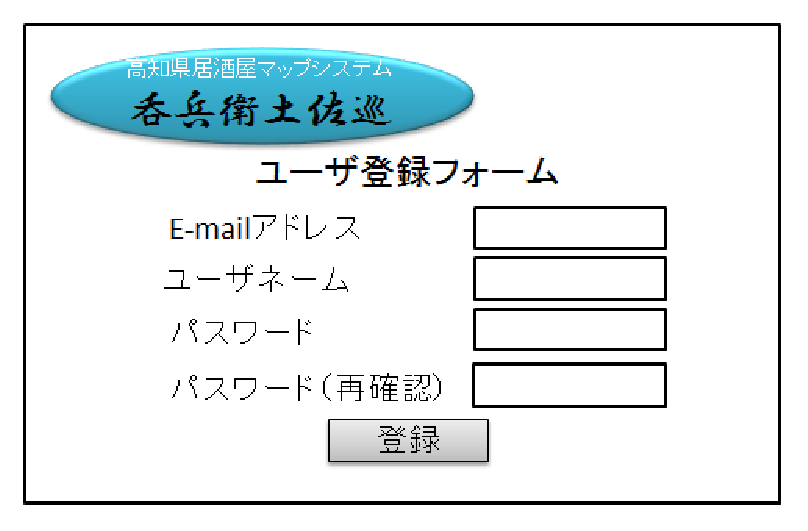
\includegraphics [height=7cm, width=7cm]{extrnal1_design_document_image/s1.eps}
  \caption{新規ユーザ登録フォーム}
  \label {fig:s1}
  \end{center}
\end{figure}

\newpage
\subsection{ユーザログイン機能}
ユーザがマイページにログインする機能です。
ユーザには、ユーザログイン画面(図\ref{fig:s2})が表示され、ログインに成功した場合はマイページ画面(図\ref{fig:s3})が表示されます。

\begin{enumerate}
  \item [入力] ユーザネーム、パスワード
  \item [出力] マイページ画面
  \item [処理] ユーザネームとパスワードをもとに、データベースからアカウント情報を取り出します
\end{enumerate}

\begin{figure}[htbp]
  \begin{center}
  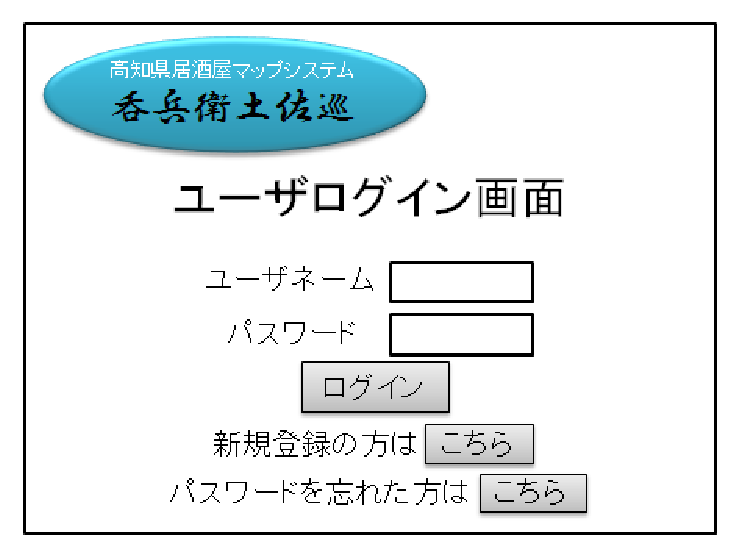
\includegraphics [height=7cm, width=7cm]{extrnal1_design_document_image/s2.eps}
  \caption{ユーザログイン画面}
  \label {fig:s2}
  \end{center}
\end{figure}

\begin{figure}[htbp]
  \begin{center}
  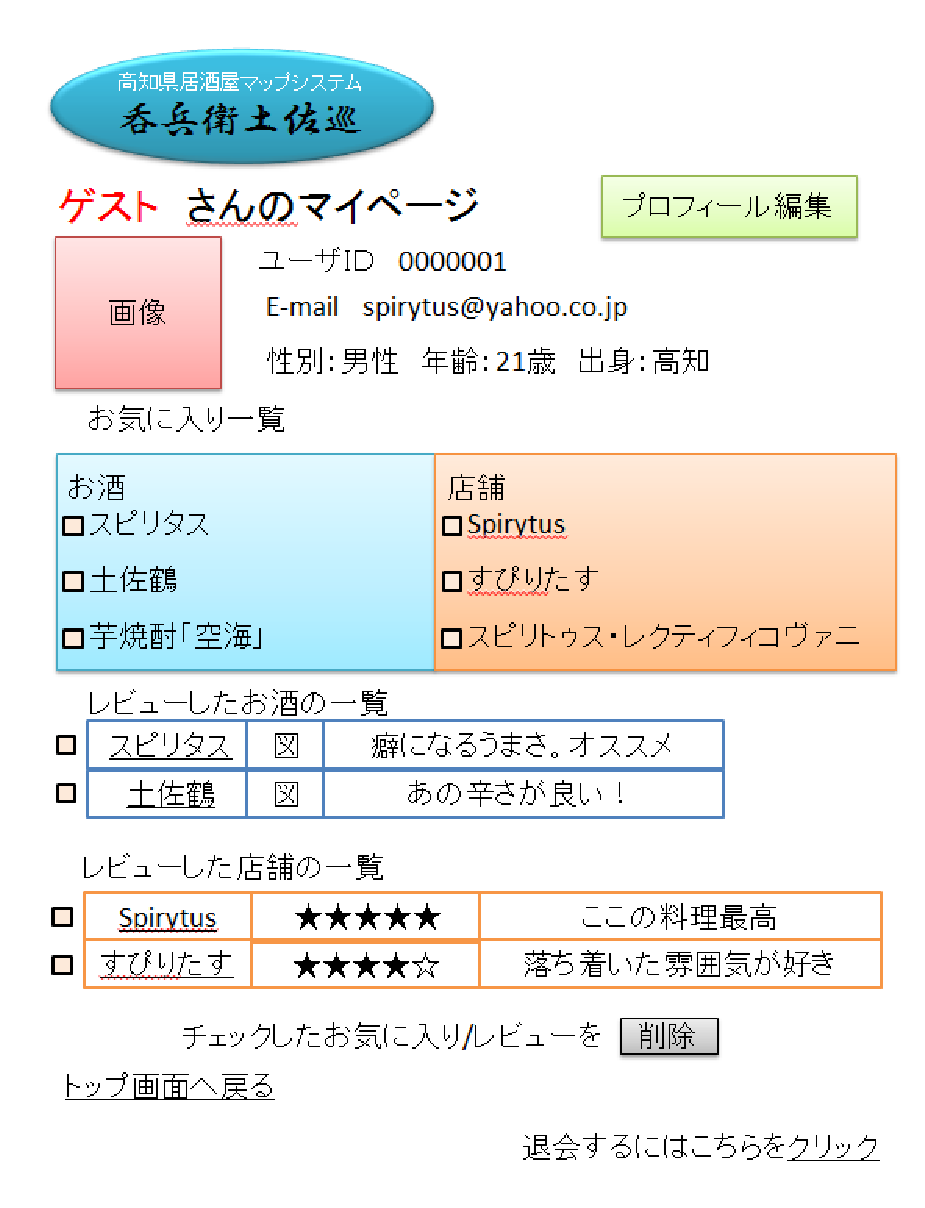
\includegraphics [height=8cm, width=6cm]{extrnal1_design_document_image/s3.eps}
  \caption{マイページ画面}
  \label {fig:s3}
  \end{center}
\end{figure}

\newpage
\subsection{店舗登録機能}
店舗側は端末を使用して店舗登録申請フォーム(図\ref{fig:s4})にアクセスし、必要情報を入力し申請を行います。
この申請に対し運営者側で店舗の広告を行うか判断します。
広告を行うと判断された場合、e-mailアドレス、パスワードをデータベースに登録します。
このe-mailアドレス、パスワードを使用しログインすることでページ編集画面にアクセスし、店舗情報の編集を行います。

\subsubsection{店舗の申請機能}
\begin{enumerate}
\item[入力] e-mailアドレス
\item[出力] メール送信
\item[処理] 登録ページのURLが記載されたメールを店舗側に送信します。店舗側はURLにアクセスし新規の登録を行い、運営側で登録された情報に対し審査を行います。登録された情報に不備等がなければそのまま登録を行います。不備等がある場合、店舗に対してメールや電話で問い合わせを行います。
\end{enumerate}

\begin{figure}[htbp]
  \begin{center}
  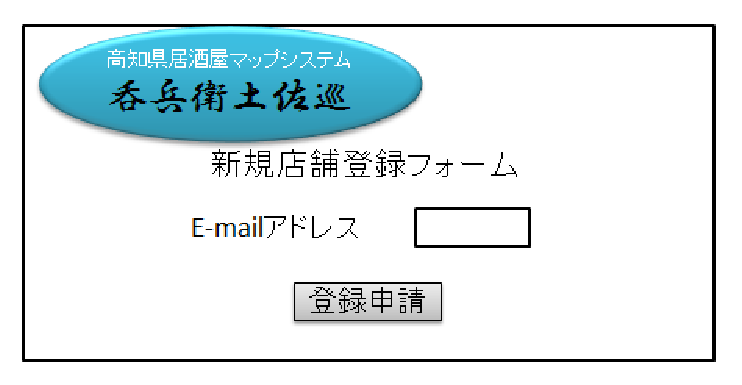
\includegraphics [height=7cm, width=7cm]{extrnal1_design_document_image/s4.eps}
  \caption{店舗登録申請フォーム}
  \label {fig:s4}
  \end{center}
\end{figure}

\newpage
\subsubsection{店舗側のログイン機能}
店舗側が店舗編集画面にログインする機能です。
店舗側には、店舗ログイン画面(図\ref{fig:s5})が表示されます。

\begin{enumerate}
\item[入力] e-mailアドレス、パスワード
\item[出力] ログイン成功ならば店舗個別ページ
\item[処理] 入力情報とデータベースを照合しログインの合否を判定します。ログインに成功した場合、店舗情報の編集画面に遷移します。
\end{enumerate}

\begin{figure}[htbp]
  \begin{center}
  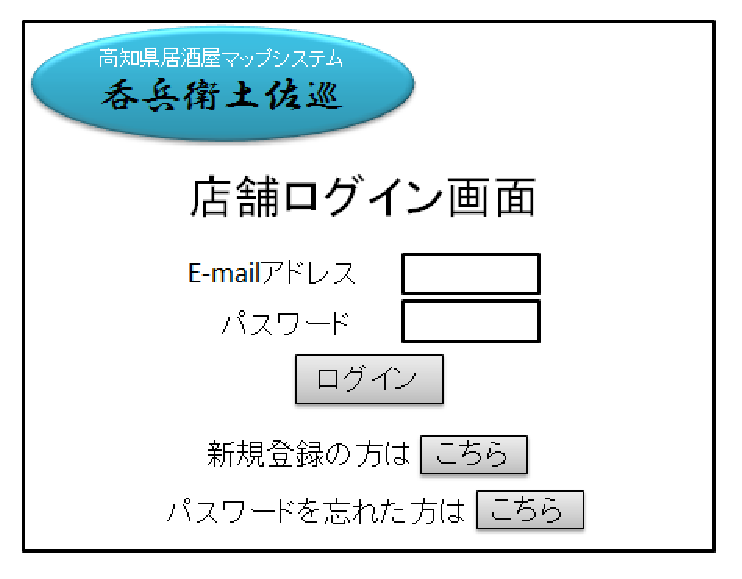
\includegraphics [height=7cm, width=7cm]{extrnal1_design_document_image/s5.eps}
  \caption{店舗ログイン画面}
  \label {fig:s5}
  \end{center}
\end{figure}

\newpage
\subsection{お酒のレビュー}
お酒の詳細情報にお酒のレビュー項目を設けています。
内容としては、ユーザIDを入力し、その選んだお酒の味を数値でレビューします。
また、コメント欄を設けお酒に対する味の感想やコメントを書いてもらいます。

\subsection{店舗のレビュー}
店舗の詳細情報に店舗のレビュー項目を設けています。
内容としては、ユーザIDを入力し、その店舗全体の雰囲気の良し悪しを数値でレビューします。
また、コメント欄を設け店舗に来た感想やコメントを書いてもらいます。
\subsection{評価基準}
レビューの評価基準としては、お酒の味・飲みやすさや店舗の雰囲気共に0〜5の6段落とし評価します。
\subsection{レビューのパラメータ}
お酒のテーブル(日本酒、ワイン、ビール等)を増やし、お酒ごとの味(甘さ・辛さ・重さ等)の評価を決めます。
\subsection{店舗側の店舗情報登録機能}
店舗情報の登録機能では上記のような店側が店舗の決められている営業時間や全体のメニュー、その他の情報を登録する機能です。
店舗側には、店舗情報登録画面(図\ref{fig:s6})が表示されます。
店舗情報入力後、画面左下の「編集確認」をクリックすることで、店舗のプレビュー画面(図\ref{fig:s7})が表示され、画面右上の「編集完了」をクリックすることで編集が完了します。

店舗情報内容
\begin{enumerate}
\item 店舗名
\item 店舗の画像
\item 営業時間(営業日の営業時間や定休日)
\item 店舗の位置(店舗の住所)
\item 交通手段(最寄の駅から車・徒歩等での所要時間)
\item 店舗の予約用電話番号(電話の際の注意事項も付け加える)
\item 座席数(個室数、カウンター数、宴会場の収容人数)
\item 喫煙席の有無
\item コースメニューの内容と値段
\item 店舗のHPやブログのURL
\item メニューと価格(お勧めだけでも)
\item 店のアピール
\end{enumerate}

\begin{figure}[htbp]
  \begin{center}
  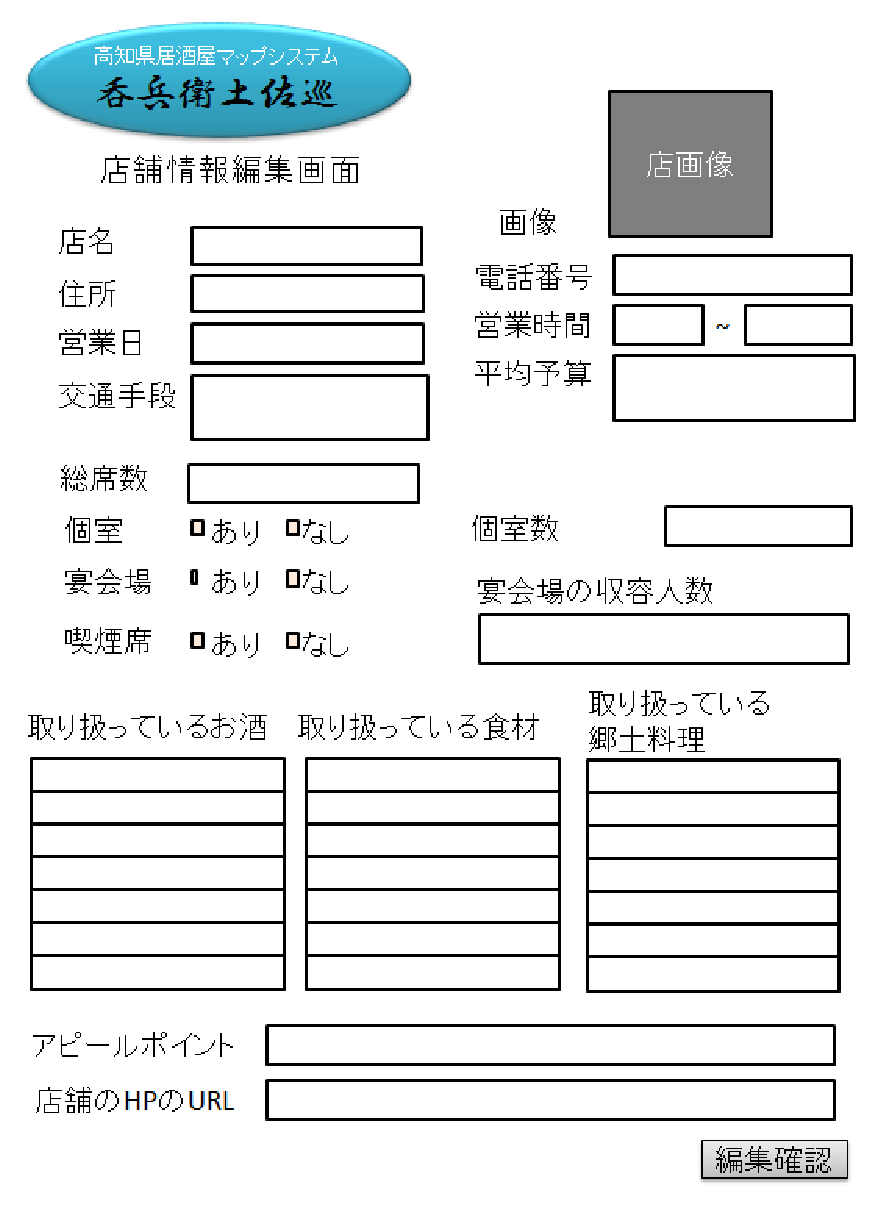
\includegraphics [height=9cm, width=6cm]{extrnal1_design_document_image/s6.eps}
  \caption{店舗情報編集画面}
  \label {fig:s6}
  \end{center}
\end{figure}

\begin{figure}[htbp]
  \begin{center}
  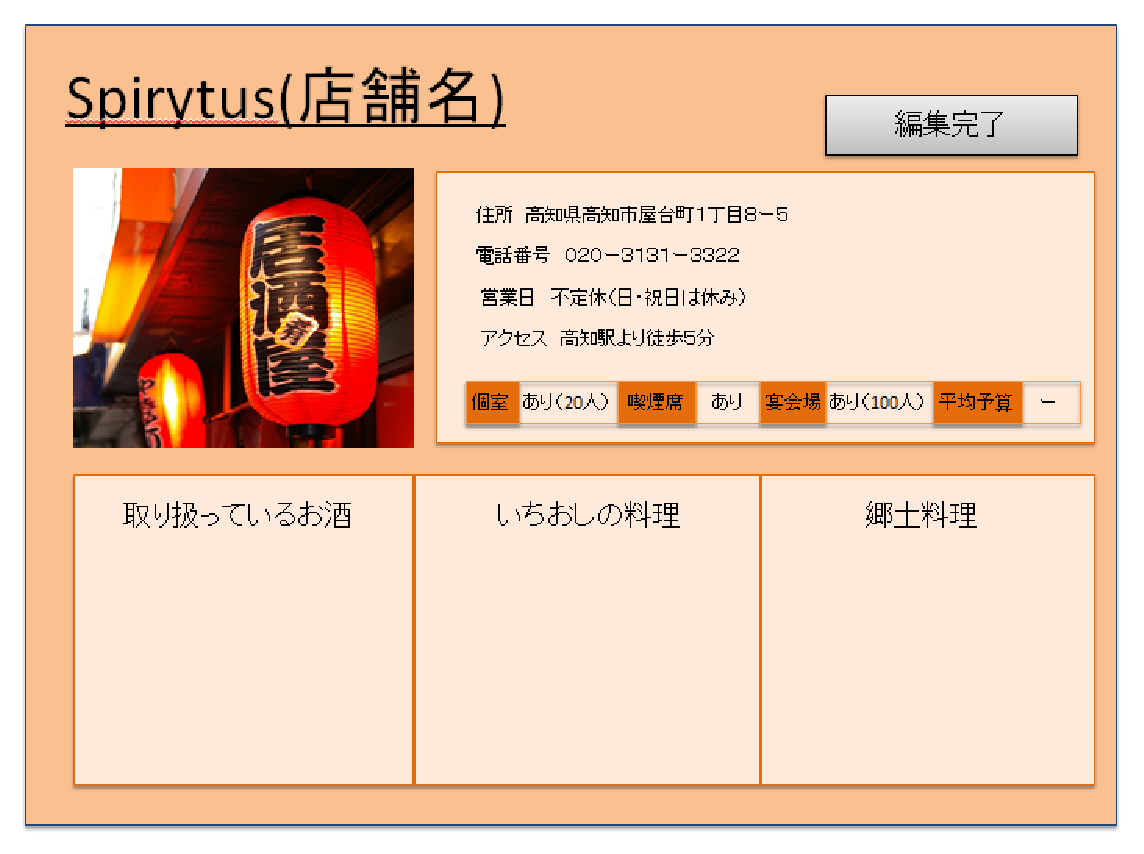
\includegraphics [height=7cm, width=7cm]{extrnal1_design_document_image/s7.eps}
  \caption{店舗のプレビュー画面}
  \label {fig:s7}
  \end{center}
\end{figure}

\newpage
\section{データ定義}
本章では、データベースで管理するデータについて定義します。
データベースのテーブルは、表\ref{tables}に示すテーブル群から構成されます。
また、これらのテーブル間のつながりを示したER図を別添ファイル「ER図.pdf」に、
各テーブルの定義を別添ファイル「データ定義書.pdf」に示します。
​
\begin{table}[!htbp]
\caption{データテーブル一覧}
\label{tables}
\begin{center}
\begin{tabular}{|l|l|l|}\hline
テーブル名 & 内容 & 詳細\\\hline\hline
liquors & お酒 & お酒に関する情報\\\hline
stores & 店舗 & 店舗に関する情報\\\hline
dishes & 料理 & 料理に関する情報\\\hline
ingredients & 食材 & 食材に関する情報\\\hline
resorts & 観光地 & 観光地に関する情報\\\hline
alcoholics & 酒類 & 酒類に関する情報\\\hline
brewers & 酒造 & 酒造に関する情報\\\hline
liquor\_reviews & お酒のレビュー & お酒のレビューに関する情報\\\hline
store\_reviews & 店舗のレビュー & 店舗のレビューに関する情報\\\hline
users & ユーザ & ユーザに関する情報\\\hline
store\_liquors & 店舗にあるお酒 & 店舗とお酒を関連付ける情報\\\hline
store\_dishes & 店舗にある料理 & 店舗と料理を関連付ける情報\\\hline
desh\_ingredients & 料理の食材 & 料理と食材を関連付ける情報\\\hline
\end{tabular}
\end{center}
\end{table}

\section{ユーザインタフェース設計}
ユーザインタフェースについては、別添ファイル「ユーザインタフェース設計書.pdf」で定義します。

\section{ネットワーク設計}
本システムは図\ref{net}のようにHTTPを用いてクライアントとサーバのやり取りを行います。
\begin{enumerate}
  \item クライアント側がサーバ側に「リクエスト」を送信します
  \item サーバ側でリクエストの解析・処理してリクエストの答えを作ります
  \item サーバ側がクライアント側に「レスポンス」を返します
\end{enumerate}
\begin{figure}[h]
  \begin{center}
    \includegraphics[width=0.8\linewidth]{net.eps}
    \caption{クライアントとサーバのやり取り}
    \label{net}
  \end{center}
\end{figure}

図\ref{server}のようにサーバを多重化することで片方のサーバに障害が発生した場合でも、もう片方のサーバでサービスを運用することが可能です。さらにデータベースのバックアップを行うことでデータの損失を防ぎます。
\begin{figure}[h]
  \begin{center}
    \includegraphics[width=0.8\linewidth]{server.eps}
    \caption{サーバの中について}
    \label{server}
  \end{center}
\end{figure}


\section{セキュリティ対策}
\subsection{不正アクセス対策}
ファイアウォールの導入により、不正アクセスが行われることを防ぎます。
また、侵入検知システム(IDS)を導入することで、
不正アクセスの兆候を検知し、早めの対応を行えるようにします。
\subsection{暗号化通信}
サーバ・クライアント間の通信は全てSSL通信を利用します。
これにより、通信内容の盗聴されることで情報が外部に漏洩することを防ぎます。
また、ユーザからの信頼性を向上させるために、SSL証明書を購入およびインストールします。
\subsection{ユーザ認証}
このシステムでは、店舗情報の登録および更新やユーザによるレビュー投稿機能を、
その権限のないユーザが行うことを防ぐために、ユーザ認証を行います。
店舗関係者とユーザのログイン時は、登録されたe-mailアドレスとパスワードの組み合わせにより認証を行います。
また、パスワードをハッシュ化してからデータベースに保存することで、
データベース内の情報が外部に漏洩してもパスワードが第三者に知られることを防ぎます。

\section{障害対策}
\subsection{ソフトウェアの障害対策}
データベースの障害対策として、メインで使用するHDD以外のHDDに、
データベースのバックアップを保存します。
毎日深夜0時に自動でバックアップを行い、
障害発生時にはこのバックアップデータからリストアし、復元します。
\subsection{許容停止時間}
障害発生によりシステムが機能しない場合、
直ちに再稼働のための手続きを行います。
システムが停止してから再稼働までの許容停止時間は48時間とします。

\section{ソフトウェア品質}
システムに組み込むプログラムは全て、テストを通過したもののみを扱います。
これにより常に一定の品質を確保します。
システムにバグが発見された場合には、直ちに修正しシステムをアップデートし、
必要に応じてテストの内容を更新します。




\end{document}
